\documentclass[11pt, english]{article}
\usepackage{graphicx}
\usepackage[colorlinks=true, linkcolor=blue]{hyperref}
\usepackage[russian,english]{babel}
\selectlanguage{russian}
\usepackage[utf8]{inputenc}
\usepackage[svgnames]{xcolor}
\usepackage{amsmath}

\usepackage{listings}
\usepackage{afterpage}
\pagestyle{plain}

\definecolor{dkgreen}{rgb}{0,0.6,0}
\definecolor{gray}{rgb}{0.5,0.5,0.5}
\definecolor{mauve}{rgb}{0.58,0,0.82}

% \lstset{language=R,
%     basicstyle=\small\ttfamily,
%   stringstyle=\color{DarkGreen},
%     otherkeywords={0,1,2,3,4,5,6,7,8,9},
%     morekeywords={TRUE,FALSE},
%     deletekeywords={data,frame,length,as,character},
%     keywordstyle=\color{blue},
%     commentstyle=\color{DarkGreen},
% }

\lstset{frame=tb,
language=java,
aboveskip=3mm,
belowskip=3mm,
showstringspaces=false,
columns=flexible,
numbers=none,
keywordstyle=\color{blue},
numberstyle=\tiny\color{gray},
commentstyle=\color{dkgreen},
stringstyle=\color{mauve},
breaklines=true,
breakatwhitespace=true,
tabsize=3
}

\usepackage{here}


\textheight=21cm
\textwidth=17cm
%\topmargin=-1cm
\oddsidemargin=0cm
\parindent=0mm
\pagestyle{plain}

%%%%%%%%%%%%%%%%%%%%%%%%%%
% La siguiente instrucción pone el curso automáticamente%
%%%%%%%%%%%%%%%%%%%%%%%%%%

\usepackage{color}
\usepackage{ragged2e}

\global\let\date\relax
\newcounter{unomenos}
\setcounter{unomenos}{\number\year}
\addtocounter{unomenos}{-1}
\stepcounter{unomenos}
\gdef\@date{\arabic{unomenos}}

\begin{document}

\begin{titlepage}

\begin{center}
\vspace*{-1in}
\begin{figure}[htb]
\begin{center}

\includegraphics[width=8cm]{bw_w_rus.png}
\end{center}
\end{figure}

Факультет Программной Инженерии и Компьютерных Технологий \\
\vspace*{0.15in}
Вычислительная математика \\
\vspace*{0.4in}
\begin{large}
ЛАБОРАТОРНАЯ РАБОТА №3\\
\end{large}
\vspace*{0.2in}
\begin{Large}
\textbf{Решение нелинейных уравнений} \\
\end{Large}
\vspace*{0.3in}
\begin{large}
Метод простых интераций \\
Метод хорд \\
\end{large}
\vspace*{0.3in}
\rule{80mm}{0.1mm}\\
\vspace*{0.1in}
\begin{large}
Преподаватель: Перл О.В. \\
Выполнил: Куприянов А.А, P3212 \\
\end{large}
\vspace*{1.5in}
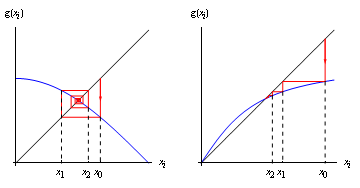
\includegraphics[width=7cm]{fixed_point_iteration_im2.png}
\\
Санкт-Петербург \\
2020
\end{center}
\end{titlepage}

\newcommand{\CC}{C\nolinebreak\hspace{-.05em}\raisebox{.4ex}{\tiny\bf +}\nolinebreak\hspace{-.10em}\raisebox{.4ex}{\tiny\bf +}}
\def\CC{{C\nolinebreak[4]\hspace{-.05em}\raisebox{.4ex}{\tiny\bf ++}}}


\section{Теория}
В ходе лабораторной работы было использовано два метода решения нелинейных уравнений: метод простых итераций и хорд

У каждого метода были выявлены свои преимущества из-за алгоритма решения уравнения.

\subsection{Метод простых итераций}
В англоязычной литературе этот метод также называется fixed point method.

Основной алгоритм метода это итеративное приближение к неподвижной точке (fixed point)

\subsubsection{Неподвижная точка}
Неподвижная точка - точка, которую заданное отображение переводит в неё же, иными словами, решение уравнения $$f(x)=x$$

\begin{figure}[h!]
    \centering
    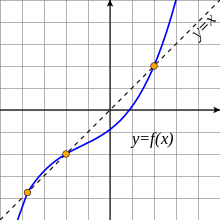
\includegraphics{fixed_point_wiki_example.png}
    \caption{Функция с тремя фиксированными точками}
    \label{fig:my_label}
\end{figure}

Простыми словами, если функция $f(x)$ пересекается с $y=x$ , то координата $x$ пересечения является фиксированной точкой

\subsubsection{Преобразование $\phi(x) = x$}
Метод простых итераций подразумевает также предварительную подготовку функции в виде проебразования $\phi(x) = x$. Зачем это нужно?
\\

Допустим, у нас имеется функция: $f(x) = x - \phi(x)$. Если мы хотим найти корни уравнения, то $f(x) = 0$. Тогда функция принимает вид: $x = \phi(x)$
\\

Это понадобится нам в ходе исполнения алгоритма

\subsubsection{Алгоритм метода простых итераций}
Условно это алгоритм можно разделить на две части: 
\begin{enumerate}
    \item Выполнить преобразование функции $f(x)$ в $\phi(x) = x$
    \item Итерировать значение $x$ к функции $\phi(x)$ до тех пор, пока не получим достаточную погрешность
\end{enumerate}
\subsubsection{Геометрическая визуализация}
Рассмотрим как это выглядит на графике
\begin{figure}[h!]
    \centering
    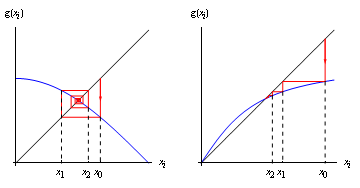
\includegraphics{fixed_point_iteration_im2.png}
    \caption{Пример итераций $x$ к функции $\phi(x)$}
    \label{fig:my_label}
\end{figure}

\subsubsection{Условие сходимости}
Мы можем сделать много функций в форме $x = \phi(x)$ из функции $f(x)$, но может ли каждая функция дать решение для $f(x)$?

Возможно. Но скорость сходимости может быть медленной.

Итак, как мы можем определить быстро ли сходится $\phi(x)$ ?
\\

Для этого мы можем проверить на условие сходимости:
\\

Если $\alpha$ решение функции $f(x)$, который эквивалентен $x = \phi(x)$ и $\alpha$ находится внутри интервала $I$ функции $\phi(x)$ и $|\phi^{'}(x)| < 1$ для любого $x \in I$. Тогда, если $x_0$ любая точка в $I$, то последовательность определенная:
$$x_n = \phi(x_{n-1}) | n \geq 1$$
будет сходится к неподвижной точке $x$ в $I$. Тогда эта неподвижная точка $x$ будет решением функции $f(x)$

\begin{figure}[h!]
    \centering
    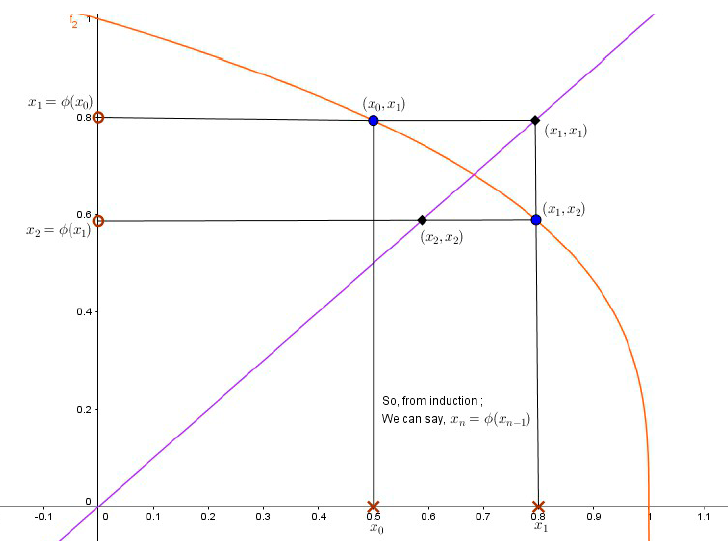
\includegraphics[height=8cm]{visualization_phi_x.png}
    \caption{Визуализация $x_n = \phi(x_{n-1})$}
    \label{fig:my_label}
\end{figure}

\subsubsection{Теорема Лагрнажа о среднем значении}
Теорема Лагранжа о среднем значении утверждает, что если функция $\phi(x)$ непрерывна на отрезке [$x_n$,$x_{n-1}$] и дифференцируема на интервале ($x_n$,$x_{n-1}$), то в этом интервале существует хотя бы одна точка $x = \epsilon$, такая что:
$$\phi(x_{n-1}) - \phi(x) = \phi^{'}(\epsilon)(x_{n-1} - x)$$

\subsubsection{Доказательство условия сходимости}
Запишем уравнение $x_n = \phi(x_{n-1})$ как $|x_n - x | = |\phi(x_{n-1}) - \phi(x)|$\\

Или применив Теорему Лагранжа можем записать:
$$|x_n - x | = |\phi^{'}(\epsilon)(x_{n-1} - x)|$$

Далее, применив неравентсво Коши-Буняковского можем прийти к виду:
$$|x_n - x | \leq |\phi^{'}(\epsilon)||(x_{n-1} - x)|$$

Положим $|\phi^{'}(\epsilon)| = k$, тогда получим:
$$|x_n - x | \leq k|(x_{n-1} - x)|$$
Индуктивно применяя неравенство мы получим:
$$|x_n - x | \leq k|(x_{n-1} - x)|$$
$$|x_n - x | \leq k*k*|(x_{n-2} - x)| = k^2|(x_{n-2} - x)|$$
$$|x_n - x | \leq k^3|(x_{n-3} - x)|$$\\
$$...$$
$$|x_n - x | \leq k^n|(x_0 - x)|$$

Предположим, что $k < 1$ и возьмем $\lim_{n\to\infty}$ :
$$\lim_{n\to\infty} |x_n - x| = \lim_{n\to\infty} k^n|x_0 - x|$$
Итого получаем:
$$\lim_{n\to\infty}|x_n - x| < 0$$
Следовательно, $\{x\}^{\infty}_{n=0}$ сходится к $x$

\subsection{Метод хорд}
\subsubsection{Метод Ньютона}
Метод Ньютона решает нелинейное уравнение $f(x) = 0$ с помощью итеративной формулы:
$$x_{i+1} = x_i - \frac{f(x_i)}{f^{'}(x_i)}$$

Минус этого метода в том, что необходиом каждый раз вычислять производную.
\subsubsection{Определение метода хорд}
Чтобы обойти это мы можем использовать апроксимацию $f(x)$ как:
$$f^{'}(x_i) = \frac{f(x_i) - f(x_{i-1})}{x_i - x_{i-1}}$$

Тогда получим:
$$x_{i+1} = x_i - \frac{f(x_i)(x_i - x_{i-1})}{f(x_i) - f(x_{i-1})}$$

Этот метод называется методом хорд. Теперь нам нужно два начальных значения, но в отличие от метода половинного деления эти два значения не должны изолировать корень.\\

Метод хорд открытый метод и может сходится или не сходится. Тем не менее, метод хорд сходится (если сходится) быстрее, чем метод половинного деления. Но так как мы апроксимировали производную из метода Ньютона, то метод хорд сходится медленнее, чем метод Ньютона.

\subsection{Метод простых итераций для системы НУ}
Для решения системы нелинейный уравнений преобразуем вводные функции к виду:
$$y = f(x)$$
$$x = \psi(y)$$

Далее, применим итерационный метод к неподвижной точке до тех пор, пока не достигнем достаточной точности
\newpage
\section{Реализация}
\subsection{Метод простых итераций}
\subsubsection{Блок схема}
\begin{figure}[h!]
    \centering
    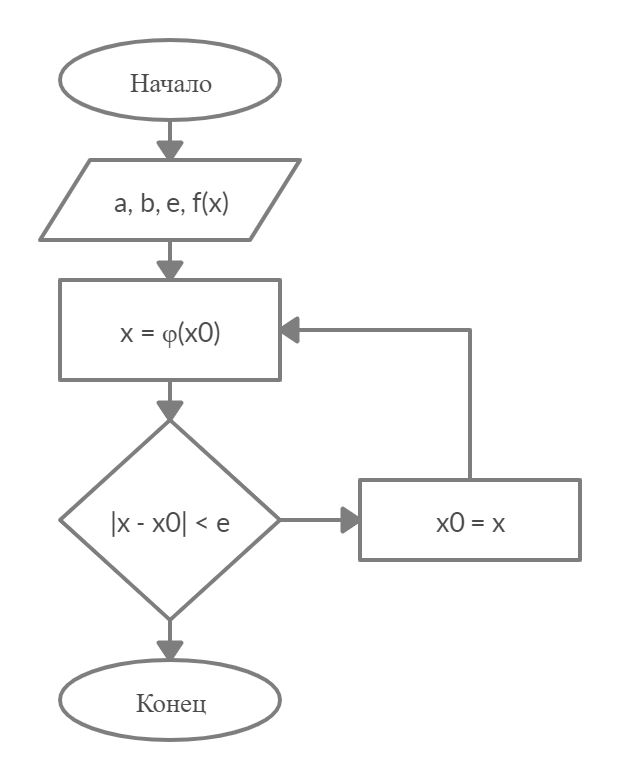
\includegraphics[width=8cm]{iterative-schema.jpg}
    \caption{Блок схема метода простых итераций}
    \label{fig:my_label}
\end{figure}
\newpage
\subsubsection{Программа на Java}

\begin{center}
    \begin{lstlisting}
    @Override
    public double solve(ExtendedFunction extFunction, double accuracy) {

        ExtendedFunction supportFunc 
                = NonLinearSolver.createSupportFunction(extFunction, accuracy);
        double x0;
        double x = extFunction.getBoundaries()[0];
        int counter = 0;
        do {
            x0 = x;
            x = supportFunc.apply(x);
            counter++;
        } while(Math.abs(x - x0) >= accuracy && counter < MAX_ITERATION);

        lastXVal = x;
        if (counter == MAX_ITERATION) {
            throw new IllegalArgumentException();
        }

        return x;
    }
    \end{lstlisting}
\end{center}
\newpage
\subsection{Метод хорд}
\subsubsection{Блок схема}
\begin{figure}[!h]
    \centering
    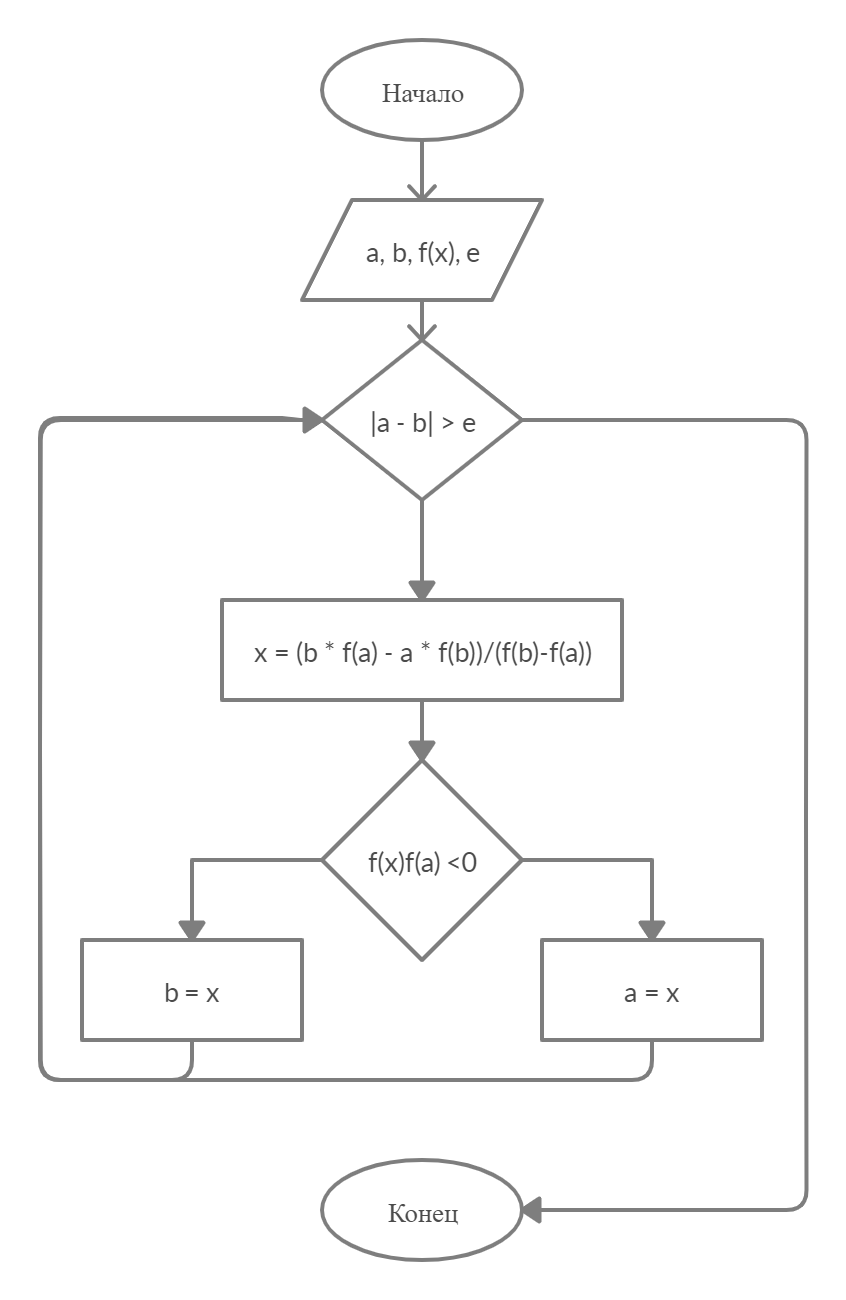
\includegraphics[width=8cm]{secant-schema.jpg}
    \caption{Блок схема метода хорд}
    \label{fig:my_label}
\end{figure}
\newpage
\subsubsection{Программа на Java}
\begin{center}
    \begin{lstlisting}
    @Override
    public double solve(ExtendedFunction extFunction, double accuracy) {

        double currentAccuracy = Double.MAX_VALUE;
        final double leftBoundary = extFunction.getBoundaries()[0];
        final double rightBoundary = extFunction.getBoundaries()[1];

        double oldValue = calculateX(extFunction, leftBoundary, rightBoundary);
        double currentValue = Double.NaN;

        int counter = MAX_DEPTH;
        while (currentAccuracy > accuracy) {

            if (isLeftSideDerivative(extFunction, oldValue)) {
                currentValue = calculateLeftSide(extFunction, oldValue);
            } else {
                currentValue = calculateRightSide(extFunction, oldValue);
            }

            currentAccuracy = Math.abs(oldValue - currentValue);
            oldValue = currentValue;

            counter--;
            if (counter  < 0 ) {
                throw new IllegalArgumentException();
            }
        }

        return currentValue;
    }

    \end{lstlisting}
\end{center}
\newpage
\begin{center}
    \begin{lstlisting}
        
    private boolean isLeftSideDerivative(ExtendedFunction function, double oldValue){
        if (function.getBoundaries()[0] < 0 && oldValue >= 0) return true;
        else return function.getBoundaries()[0] >= 0 && oldValue < 0;
    }

    private double calculateRightSide(ExtendedFunction function, double oldValue){
        return calculateX(function, oldValue, function.getBoundaries()[1]);
    }

    private double calculateLeftSide(ExtendedFunction function, double oldValue) {
        return calculateX(function,function.getBoundaries()[0], oldValue);
    }

    private double calculateX(ExtendedFunction func, double a, double b) {
        final double funcA = func.apply(a);
        final double funcB = func.apply(b);
        return (a * funcB - b * funcA) / (funcB - funcA);
    }
    \end{lstlisting}
\end{center}
\newpage
\subsection{Метод простых итераций для решения систем НУ}
\subsubsection{Блок схема}
\begin{figure}[h!]
    \centering
    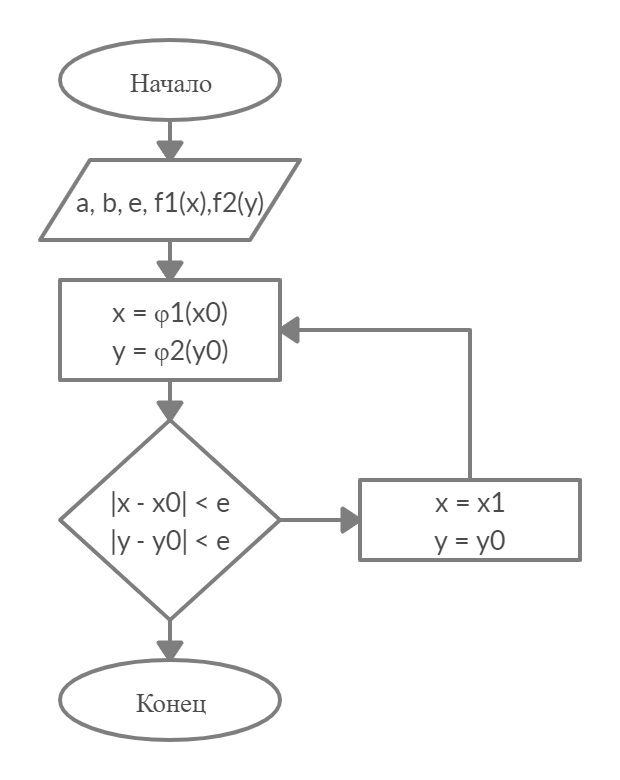
\includegraphics[width=8cm]{schema-3.jpg}
    \caption{Метод итераций для НУ}
    \label{fig:my_label}
\end{figure}
\newpage
\subsubsection{Программа на Java}
\begin{center}
    \begin{lstlisting}
    @Override
    public double[] nonlinearSystemSolver(List<ExtendedFunction> functions, double accuracy) {
        List<Double> rootList = new ArrayList<>();
        for (int i = 0; i < functions.size(); i++) {
            rootList.add(i, functions.get(i).getBoundaries()[0]);
        }
        List<Double> listX0 = new ArrayList<>(rootList);
        int counter = 0;
        do {
            for (int i = 0; i < functions.size(); i++) {
                ExtendedFunction supportFunc = functions.get(i);
                listX0.set(i, rootList.get(i));
                rootList.set(i, supportFunc.apply(rootList.get(i)));
                if (Math.abs(functions.get(0).getDerivativeFunction().apply(rootList.get(0))) > 1 && Math.abs(functions.get(1).getDerivativeFunction().apply(rootList.get(1))) > 1) {
                    throw new IllegalArgumentException();
                }
                for (double d : rootList) if (Double.isInfinite(d)) throw new IllegalArgumentException();
                counter++;
            }
        } while(allInListDeltaMoreThanAccuracy(rootList, listX0, accuracy) && counter < MAX_ITERATION);

        return new double[]{rootList.get(1), rootList.get(0)};
    }

    private boolean allInListDeltaMoreThanAccuracy(List<Double> listX, List<Double> listX0, double accuracy){

        boolean moreThanAccuracy = false;
        for (int i = 0; i < listX.size(); i++) {
            double x = listX.get(i);
            double x0 = listX0.get(i);
            moreThanAccuracy = Math.abs(x - x0) >= accuracy;
        }
        return moreThanAccuracy;
    }
    \end{lstlisting}
\end{center}
\section{Заключение}
Использование двух методов дало возможность сравнить их особенности и реализации. \\

Как уже говорилось метод хорд является упрощением метода Ньютона, что достигается за счёт апроксимации производной в формуле метода Ньютона. Из-за этого сходимость данного метода ниже, чем у оригинального метода Ньютона, тем не менее, быстрее, чем метод половинного деления. \\

А метод простых итераций был достаточно интересным с математической точки зрения, так как основой данного метода является преобразование исходный функции в функцию вида:
$$x = \phi(x)$$
Совершенно нетривиальный итеративный метод решения. \\
% Здесь вторая часть ...%

Также в этой работе была не только имплементация вычислительных методов, но и создание GUI для отображения графиков. Я решил не использовать UI библиотеки и написать сам строитель графиков на технологии Swing Java.
\end{document}